\documentclass[12pt]{article}
\usepackage[utf8]{inputenc}
\usepackage{blindtext}
\usepackage{fancyhdr}
\usepackage{graphicx}
\usepackage{amsmath}
\usepackage{amssymb}
\usepackage[table,xcdraw]{xcolor}
\usepackage{float}
  \usepackage{setspace}
\usepackage{geometry}
 \geometry{
 a4paper,
 left=20mm,
 right=20mm,
 bottom=25mm,
 top=25mm,
 }
 \usepackage[
backend=biber,
style=mla-new,
citestyle=authoryear
]{biblatex}
\addbibresource{sources.bib}
 
 \newcommand{\icol}[1]{% inline column vector
  \left(\begin{smallmatrix}#1\end{smallmatrix}\right)%
}
 
\pagestyle{fancy}
\fancyhf{}
\lhead{Research Question: How fast should a camera rotate to record a zipliner traveling at constant velocity in the center of the frame? }
\rfoot{Page \thepage}

\doublespacing
\begin{document}
\begin{titlepage}
   \begin{center}
        \vspace*{5cm}

        \Huge{Related Rates of a Camera Videotaping Zipliners}

        \vspace{1cm}
        \LARGE{How fast should a camera rotate to record a zipliner traveling at constant velocity in the center of the frame?}
            
        \vspace{2 cm}
        \Large{IB Code \#}
        
        \vspace{0.5 cm}
        \large{18 Pages}
       
        \vspace{2cm}
        \large{IB Mathematics Analysis and Approaches Higher Level}
       
        \vspace{1 cm}
        \Large{Internal Assessment}
       

       \vfill
    \end{center}
\end{titlepage}
    
\tableofcontents
\newpage
    
\section{Introduction}
My uncle owns a zipline park in Yucatan, Mexico, which is mostly visited by tourists for the stunning views. Tourists have often wanted to have videos taken of them, but there is currently no implementation of a camera to record them. Videos taken from stationary viewers often fail to smoothly track the motion of the zipliners, resulting in bad-quality videos and no memories from the zipline. I saw this as an opportunity to position a mechanical motor with a camera which will rotate to record the entire ride of the zipliners, from start to finish. 

\subsection{Rationale}
This investigation will explore how such a camera could be programmed to rotate in all three dimensions to follow the zipliner at all times along their rides. At its core, this will be a related rates problem, however, due to its 3-dimensional nature, it will require an in-depth application of vectors. Ultimately, I want to find how fast each of the three motors spinning the camera should rotate to track the zipliner at all times, assuming that the zipliner travels at constant velocity. Since there are several ziplines at the park and many places to position the camera for different background views, I want to find a general solution to the rates of change of the angles for any zipline in the park with a camera at any point. I will then apply it to one of the smaller ziplines that has a beautiful view over a river. 

\subsection{Aim}
To answer the question "How fast should a camera rotate to record a zipliner traveling at constant velocity in the center of the frame?", I will find equations for the rates of change of the angles defining the orientation of the camera over time as the zipliner travels down the zipline. 

\section{Defining the Problem}

I will position the camera next to the zipline on a stand at the same height as the end of the zipline, and want it to rotate in such a way that it tracks the zipliner as they ascend. I will define the following variables, which are the given variables for any zipline. I have also found the values of each variable for the zipline I will be recording. In this scenario, I set up the camera as the origin for improved readibility when doing the calculations.

% variable stuff // meaning // application

\begin{table}[H]
\centering
\begin{tabular}{|l|l|l|}
\hline
\rowcolor[HTML]{C0C0C0} 
Variable     & Meaning                                                                                      & Real Value \\ \hline
$P_i(x_i,y_i,z_i)$ & \begin{tabular}[c]{@{}l@{}}Point where the zipline starts\\ and its coordinates in meters\end{tabular} & $P_i(24,28,11)$    \\ \hline
$P_f(x_f, y_f, z_f)$ & \begin{tabular}[c]{@{}l@{}}Point where the zipline ends \\ and its coordinates in meters\end{tabular}  & $P_f(-28,8,0)$  \\ \hline
$C(x_c, y_c, z_c)$ & \begin{tabular}[c]{@{}l@{}}Point where camera is and \\ its coordinates in meters\end{tabular}  &  $C(0,0,0)$  \\ \hline
$\vec v = v_x\vec i + v_y\vec j + v_z \vec k$ & \begin{tabular}[c]{@{}l@{}}Velocity vector of zipliner \\ assuming constant velocity \\ in meters per seconds squared \end{tabular}  &  $\vec v = -5.2\vec i - 2\vec j - 1.1 \vec k$  \\ \hline
$t$ & \begin{tabular}[c]{@{}l@{}}Time (in seconds) since \\ the zipliner began traveling \end{tabular}  &  \begin{tabular}[c]{@{}l@{}}Duration of zipline, \\ found later \end{tabular}  \\ \hline
\end{tabular}
\end{table}

It would be helpful to find the coordinates of the point at which the zipliner is currently located as a function of time. Expressing this point, let's call it $P_c$, as a vector, $\vec P_c$, we have the following equation for it using the line of the zipline, 

$$\vec P_c = \begin{pmatrix} x_i \\ y_i \\ z_i \\ \end{pmatrix} + t\begin{pmatrix} v_x \\ v_y \\ v_z \\ \end{pmatrix}$$
Or, simply changing it to point-coordinate form to stay consistent with the above table, 
$$P_c(x_i+tv_x, y_i+tv_y, z_i+tv_z)$$


Using the points from the table above, let's define the following vectors and their magnitudes.

$$
\begin{array}{c|c}
     \overrightarrow{P_iP_c} = \begin{pmatrix} tv_x \\ tv_y \\ tv_z \\ \end{pmatrix} & \text{(Zipline vector)} \\ \\
     D = \left\lvert \overrightarrow{P_iP_c} \right\rvert = t \sqrt{v_x^2 + v_y^2 + v_z^2} & \text{(Distance traveled by zipliner)} \\ 
     
\end{array}
$$

$$
\begin{array}{c|c}
     \overrightarrow{CP_i} = \begin{pmatrix} x_i - c_x \\ y_i - c_y \\ z_i - c_z \\ \end{pmatrix} & \text{(Initial camera orientation vector)} \\ \\
     L = \left\lvert \overrightarrow{CP_i} \right\rvert = \sqrt{(x_i-c_x)^2 + (y_i-c_y)^2 + (z_i-c_z)^2} & \text{(Camera to zipline start distance)} \\
     
\end{array}
$$

\section{Finding an Equation for Each Angle}

Now we can begin searching for equations defining the orientation of the camera. To do that, we first have to define what we mean by the camera 'following' the zipliner. This means that the camera's line of sight will always be pointing at the zipliner, thus keeping them in the center of the frame at all times. We can call this line of sight vector $\vec n$, which is actually the vector between the points $C$ and $P_c$. Hence, we can define the following.
$$\vec n = \overrightarrow{CP_c} = \begin{pmatrix} x_i + tv_x - c_x \\ y_i + tv_y - c_y \\ z_i + tv_z - c_z \\
\end{pmatrix} = \begin{pmatrix} x_t \\ y_t \\ z_t \\
\end{pmatrix}$$

Now that we know that by the camera's orientation is defined by the vector $\vec n$, let's find the angles that define the direction of this vector, in radians, which the mechanical motors will use to rotate into those directions to position the camera in the direction of $\vec v$. Since I ultimately want to find an angle, I will define the orientation of the vector using the angles between it and the x-axis, y-axis, and z-axis. I can then set up my motors to rotate the camera along those axis to follow the current position of the zipliner. To do that, let's define the unit vectors of each axis in the three dimensions, 


$$\vec x = \begin{pmatrix} 1 \\ 0 \\ 0 \\
\end{pmatrix}, \quad \vec y = \begin{pmatrix} 0 \\ 1 \\ 0 \\
\end{pmatrix}, \quad \vec z = \begin{pmatrix} 0 \\ 0 \\ 1 \\ \end{pmatrix}$$

Now, let's define the following angles which will be the focus of this investigation. We ultimately want to find their rates of change across time.
$$
\begin{array}{lc}
 \theta_x & \text{(Angle, in radians, between } \vec x \text{ and } \vec n \text{)}\\
 \theta_y & \text{(Angle, in radians, between } \vec y \text{ and } \vec n\text{)}\\
 \theta_z & \text{(Angle, in radians, between } \vec z \text{ and } \vec n\text{)}\\
\end{array}
$$

I constructed the following diagram in Figure 1 to demonstrate the meaning of each angle. As shown, the angles define the orientation of the camera, and therefore will be used to position the camera in such a way that it follows the zipliner.

\begin{figure}[H]
\centering
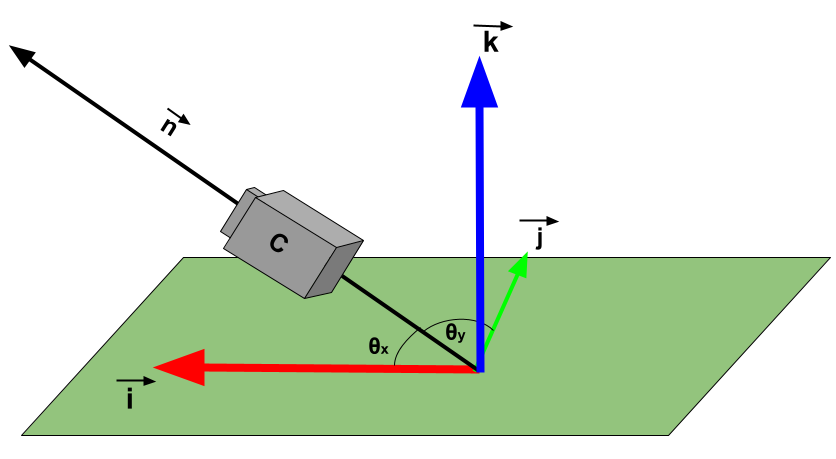
\includegraphics[width=400pt]{img/angles.png}
\caption{\label{fig:1}Diagram of Camera's Rotation}
\end{figure}

To find these angles, I will use the dot product between the line of sight of the camera, $\vec n$, and each orthogonal line. This will produce an equation relating the cosine of the angle and the distance between the camera, since the orthogonal vectors $\vec x$, $\vec y$, and $\vec z$ are all unit vectors. Although I am finding equations for the related rates of all three angles, I will begin by finding the equation for $\theta_x$, and then show the final equations for $\theta_y$ and $\theta_z$ for conciseness.

$$
\begin{array}{c|c}
 \vec n \cdot \vec x = \mid \vec n \mid \mid \vec x \mid \cos \theta_x & \text{(Dot product equation)} \\
 \rightarrow (x_t)(1) + (y_t)(0) + (z_t)(0) = \mid \vec n \mid \cos \theta_x & \text{(Calculate dot product)} \\ \\
 \boxed{\rightarrow \cos \theta_x =  \frac{x_t}{\mid \vec n \mid}} & \text{(Solve for cosine of angle)}\\ \\
 \boxed{\rightarrow \cos\theta_y =  \frac{y_t}{\mid \vec n \mid}} & \text{(Similar equation for y angle)}\\ \\
 \boxed{\rightarrow \cos \theta_z = \frac{z_t}{\mid \vec n \mid}} & \text{(Similar equation for z angle)} \\
\end{array}
$$


These three equations relate the angles defining the orientation of the camera and the vector between the camera and position of the zipliner.


\section{Finding Rates of Change of Angles}

We can now move on to finding the rates of change of the equations for the angles found in the previous section. As before, I will begin by solving for $\dfrac{d\theta_x}{dt}$, and then show the similar equations that I derived for $\dfrac{d\theta_y}{dt}$ and $\dfrac{d\theta_z}{dt}$ for conciseness.
$$\frac{d}{dt}\cos \theta_x = \frac{d}{dt} \frac{x_t}{\sqrt{x_t^2+y_t^2+z_t^2}} \quad \quad \text{(Differentiate both sides)}$$

Evaluating the derivative of the right-hand side will involve multiple steps, so I will use multiple substitutions to improve readability and ensure I do not commit any errors.

First, let's find the following derivatives that we can substitute later, 
$$\frac{d}{dt} x_t = \frac{d}{dt} (x_i + tv_x - c_x) = v_x$$
$$\text{Similarly, }\frac{d}{dt} y_t = v_y \text{ and }\frac{d}{dt} z_t = v_z$$

Now, in preparation for the chain rule, let's use the u-substitution method to find the derivative of $\mid \vec n \mid$ using what we know from basic differentiation. I found it interesting how there is an opportunity to delve into vector calculus at this stage. There are distinct rules for differentiating vectors and their magnitudes within multi-variable calculus \autocite{multivar}. However, I will instead expand the vectors into their components and use the calculus within the curriculum, although this is definitely an extension that could improve the readability of the investigation and provide deeper insight into the operations that follow. 

% SOURCE; https://ocw.mit.edu/resources/res-18-007-calculus-revisited-multivariable-calculus-fall-2011/study-materials/MITRES_18_007_supp_notes03.pdf

$$
\begin{array}{c|c}
 \text{let } u = \sqrt{x_t^2+y_t^2+z_t^2} & \text{(Note how }u=\mid \vec n \mid \text{)} \\ \\
 \dfrac{d}{dt} u = \dfrac{1}{2\sqrt{x_t^2+y_t^2+z_t^2}}(2x_tv_x + 2y_tv_y + 2z_tv_z) & \text{(Chain rule)}
\end{array}
$$
\\
At first, looking at this derivative, I thought the final equation was going to be extremely long and messy. This would have resulted in a lengthy, illegible final equation. However, I realized a pattern in the equation for $\frac{du}{dt}$ that resembled a dot product of $\vec n \cdot \vec v$. Rewriting it using vector operations drastically simplifies the equation and makes it concise. Written in terms of a scalar product, we are able to view a glimpse of vector calculus through the derivative of the magnitude of vector $\vec n$. I found the simplicity of this derivative beautiful, and find it exciting that I just proved a rule of vector calculus using ordinary differentiation. 


$$\frac{du}{dt} = \frac{\vec n \cdot \vec v}{\mid \vec n \mid} \quad \quad \text{(Rewrite in terms of dot product)}$$

Finally, let's evaluate the right hand side of the equation, then substitute it back into the differentiated equation to find the rate of change of $\theta_x$.

$$
\begin{array}{l|c}
  \dfrac{d}{dt}\dfrac{x_t}{u} & \text{(First, let's calculate RHS)} \\ \\
  =\dfrac{u\dfrac{dx_t}{dt} - x_t\dfrac{du}{dt}}{u^2} & \text{(Use quotient rule)} \\ \\
 
\end{array} 
$$

$$
\begin{array}{l|c}
  =\dfrac{\mid \vec n \mid v_x - x_t\left(\dfrac{\vec n \cdot \vec v}{\mid \vec n \mid}\right)}{{\mid \vec n \mid}^2} & \text{(Substitute known derivatives)} \\ \\
  =\dfrac{{\mid \vec n \mid}^2 v_x -x_t (\vec n \cdot \vec v)}{{\mid \vec n \mid}^3} & \text{(Simplify fraction with } \mid \vec n \mid \text{)} \\ \\
  \therefore \dfrac{d\theta_x}{dt}(-\sin  \theta_x) = \dfrac{{\mid \vec n \mid}^2 v_x - x_t(\vec n \cdot \vec v)}{{\mid \vec n \mid}^3} & \text{(Substitute into original equation)} \\ \\
  \boxed{\rightarrow \frac{d\theta_x}{dt} = \frac{{\mid \vec n \mid}^2 v_x - x_t(\vec n \cdot \vec v)}{-\sin  \theta_x{\mid \vec n \mid}^3}} & \text{(Equation for } \dfrac{d\theta_x}{dt} \text{)}   \\

\end{array} 
$$


Similarly, we arrive at the equations for the rates of change of the other two angles, 

$$\boxed{\rightarrow \frac{d\theta_y}{dt} = \frac{{\mid \vec n \mid}^2 v_y - y_t(\vec n \cdot \vec v)}{-\sin  \theta_y{\mid \vec n \mid}^3}} \quad \quad \text{(Similar equation for } \theta_y \text{)}$$

$$\boxed{\rightarrow \frac{d\theta_z}{dt} = \frac{{\mid \vec n \mid}^2 v_z - z_t(\vec n \cdot \vec v)}{-\sin  \theta_z{\mid \vec n \mid}^3}} \quad \quad \text{(Similar equation for } \theta_z \text{)}$$



\section{Simplifying Unknown Variables}

Although we found the equations we were looking for, it would be nice if they were only in terms of $\vec n$. To do that, let's expand all other variables in the equations and simplify, beginning with $\sin \theta_x$, which I can find using the cross product of vector $\vec n$ and the orthogonal line between which we are measuring the angle, in this case $\vec x$.

$$
\begin{array}{l|c}
 \mid \vec n \times \vec x \mid = \mid \vec n \mid \mid \vec x \mid \sin \theta_x & \text{(Cross product equation)}\\ \\
 \rightarrow \sin \theta_x = \dfrac{\mid \vec n \times \vec x \mid}{\mid \vec n \mid} & \text{(Solve for } \sin \theta_x \text{)} \\
\end{array} 
$$


I realized that expanding the cross product could result in an even more concise equation for $\dfrac{d\theta_x}{dt}$. Let's calculate this,

$$
\begin{array}{l|c}
 \vec n \times \vec x = \begin{pmatrix} x_t \\ y_t \\ z_t \\
\end{pmatrix} \times \begin{pmatrix} 1 \\ 0 \\ 0 \\
\end{pmatrix} & \text{(Expand into component vectors)}\\ \\
=\begin{pmatrix} y_t(0) - z_t(0) \\ z_t(1) - x_t(0) \\ x_t(0) - y_t(1) \\
\end{pmatrix} & \text{(Calculate cross product)}\\ \\
= \begin{pmatrix} 0 \\ z_t \\ -y_t \\ 
\end{pmatrix} & \text{(Cross product vector)} \\ \\
\therefore \mid \vec n \times \vec x \mid = \sqrt{0^2 + z_t^2 +(-y_t)^2} & \text{(Calculate magnitude)} \\ \\
= \sqrt{z_t^2 + y_t^2} & \text{(Magnitude of cross product)} \\ \\
\boxed{\therefore \; \sin \theta_x = \frac{\sqrt{z_t^2 + y_t^2}}{\mid \vec n \mid}} & \text{(Substitute into } \sin \theta_x \text{)} \\ \\
\boxed{\therefore \; \sin \theta_y = \frac{\sqrt{x_t^2 + z_t^2}}{\mid \vec n \mid}} & \text{(Similar equation for y angle)} \\ \\
\boxed{\therefore \; \sin \theta_z = \frac{\sqrt{x_t^2 + y_t^2}}{\mid \vec n \mid}} & \text{(Similar equation for z angle)} \\
\end{array} 
$$

\vspace{20pt}
These values can now be substituted into $\sin \theta_x$ of the original related rates equation to achieve final equations for the rates of change of the three angles only in terms of vector $\vec n$ and its components so that it can be easily evaluated.

$$
\begin{array}{l|c}
 \dfrac{d\theta_x}{dt} = \dfrac{{\mid \vec n \mid}^2 v_x - x_t(\vec n \cdot \vec v)}{-(\dfrac{\sqrt{z_t^2 + y_t^2}}{\mid \vec n \mid}) {\mid \vec n \mid}^3} & \text{(Substitute } \sin \theta_x \text{)} \\ \\
 \rightarrow \dfrac{d\theta_x}{dt} = \dfrac{ x_t(\vec n \cdot \vec v) - {\mid \vec n \mid}^2 v_x}{\sqrt{z_t^2 + y_t^2} {\mid \vec n \mid}^2} & \text{(Simplify)} \\ \\
 \end{array} 
$$
\newline
\begin{equation}
    \boxed{\therefore \frac{d\theta_x}{dt} = \frac{x_t(\vec n \cdot \vec v) - {\mid \vec n \mid}^2 v_x}{\sqrt{z_t^2 + y_t^2} {\mid \vec n \mid}^2}}  \quad \text{(Angle rotated from x axis)}
\end{equation}

\begin{equation}
    \boxed{\therefore \frac{d\theta_y}{dt} = \frac{y_t(\vec n \cdot \vec v) - {\mid \vec n \mid}^2 v_y}{\sqrt{x_t^2 + z_t^2} {\mid \vec n \mid}^2}} \quad \text{(Angle rotated from y axis)}
\end{equation}

\begin{equation}
    \boxed{\therefore \frac{d\theta_z}{dt} = \frac{z_t(\vec n \cdot \vec v) - {\mid \vec n \mid}^2 v_z }{\sqrt{x_t^2 + y_t^2} {\mid \vec n \mid}^2}} \quad \text{(Angle rotated from z axis)}
\end{equation}

$$\text{Where, as a reminder, } \vec n = \overrightarrow{CP_c} = \begin{pmatrix} x_t \\ y_t \\ z_t \\ \end{pmatrix} = \begin{pmatrix} x_i-c_x+tv_x \\ y_i-c_y + tv_y \\ z_i-c_z + tv_z \\ \end{pmatrix}$$

Meaning that, ultimately, the three rates of change are in terms of the four given values in the beginning of the problem: points $P_i$, $C$, $\vec v$, and time $t$. However, I will not expand $\vec n$ so that the equations remain concise while also providing insight into the meaning of the vectors being calculated.

I think its worth reflecting on these equations and their uncanny similarity. There is a beautiful pattern that each follows with striking resemblance. This boils down to their relationship through vector calculus. What I find amazing is that even without vector calculus, instead expanding each vector into its components, I was able to achieve such elegant solutions with clear, repeating structure. Enough about its beauty, time to set up my Uncle's zipline camera!

\section{Application}

As a reminder, the following are the given variables for the zipline I will be videotaping.
$$
\begin{array}{c|c}
    P_i(24,28,11), \quad P_f(-28,8,0), \quad C(0,0,0) & \text{(in }m\text{)} \\
    \vec v = -5.2\vec i - 2\vec j -1.1 \vec k & \text{(in } \dfrac{m}{s^2} \text{)}  
\end{array}
$$

I additionally constructed the following 3-dimensional graph to visualize the three points, which could also help us understand the angle measurements later on. 
\begin{figure}[H]
\centering
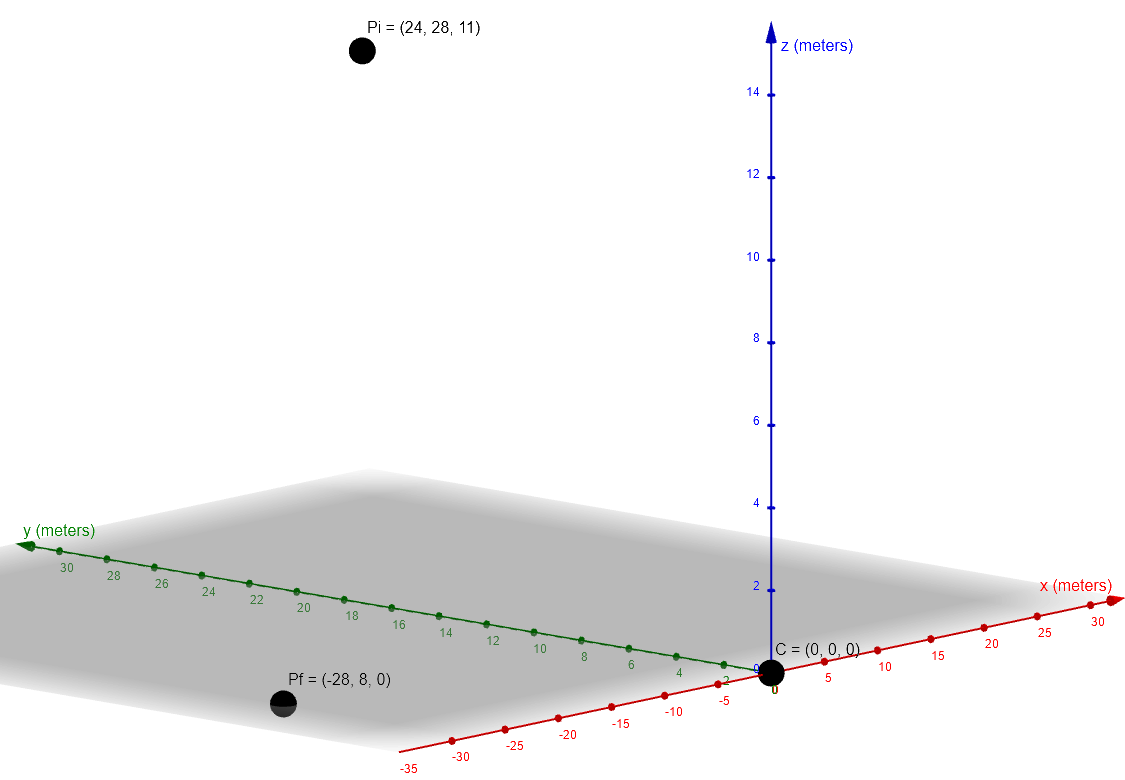
\includegraphics[width=300pt]{img/geogebra1.png}
\caption{\label{fig:2}3-Dimensional Graph Showcasing zipline Points and Camera Point}
\end{figure}


\subsection{Finding the Rates of Change}

Since we kept the equations for the rates of change of the angles in terms of vector $\vec n$ and its components, let's begin by evaluating this vector. Recalling that the current position vector of the zipliner is defined by the following line, we can proceed to find $\vec n$ in terms of time $t$.

$$\vec P_c =  \begin{pmatrix} 24 \\ 28 \\ 11 \\ \end{pmatrix} + t \begin{pmatrix} -5.2 \\ -2 \\ -1.1 \\ \end{pmatrix}$$
\newpage
Now, let's evaluate $\vec n$.

$$
\begin{array}{c|c}
    \vec n = \overrightarrow{CP_c} =  \begin{pmatrix} 24 -5.2t - 0 \\ 28 -2t - 0 \\ 11-1.1t -0 \\ \end{pmatrix} & \text{(Vector between camera and zipliner)} \\ \\
    \begin{cases}
      x_t = 24-5.2t \\
      y_t = 28-2t \\
      z_t = 11-1.1t 
    \end{cases} & \text{(Parametric Equations)} \\
 \end{array} 
$$

Using this information, let's evaluate the magnitude of the vector so that we can substitute it into the equations for the rates of change. 
$$
\begin{array}{l|c}
    \mid \vec n \mid = \sqrt{(24-5.2t)^2+(28-2t)^2+(11-1.1t)^2} & \text{(Magnitude in terms of time)} \\
    = \sqrt{32.25t^2 - 385.8t + 1481} & \text{(Simplify)} \\
 \end{array} 
$$

Next, let's find the dot product $\vec n \cdot \vec v$ since this expression appears in all three equations.

$$
\begin{array}{l|c}
    \vec n \cdot \vec v & \text{(Dot product)} \\
    = -5.2(24-5.2t) - 2(28-2t) - 1.1(11-1.1t) & \text{(Expand)}\\
    = 32.25t-192.9& \text{(Simplify)}\\
 \end{array} 
$$

\vspace{20pt}
Now, we are ready to solve for the rates of change, beginning with angle $\theta_x$ using the equation previously derived.

While the equations will appear more complex than I expected, this is understandable as the angle about each axis depends on all three dimensions, therefore will not linearly increase or decrease even if the zipliner is moving in a straight line. Moreover, I find that the equations resembled a beautiful pattern and structure in their vector form which is lost when solving for time. However, this way of expressing it, although sacrificing the meaning behind each vector, allows us to understand the angle across time as the only variable! 

$$
\begin{array}{l|c}
    \dfrac{d\theta_x}{dt} = \dfrac{x_t(\vec n \cdot \vec v) - {\mid \vec n \mid}^2 v_x}{\sqrt{z_t^2 + y_t^2} {\mid \vec n \mid}^2} & \text{(Using Equation 1)} \\ \\
    = \dfrac{(24-5.2t)(32.25t-192.9) - \left(\sqrt{32.25t^2 - 385.8t + 1481}\right)^2 (-5.2)}{\sqrt{(11-1.1t)^2 + (28-2t)^2} \left( \sqrt{32.25t^2 - 385.8t + 1481}\right)^2} & \text{(Substitute values)}\\ \\
    = \dfrac{(24-5.2t)(32.25t-192.9) + 5.2(32.25t^2 - 385.8t + 1481)}{\sqrt{(11-1.1t)^2 + (28-2t)^2} (32.25t^2 - 385.8t + 1481)} & \text{(Simplify)}\\ \\
    = \dfrac{-229.08t+3071.6}{\sqrt{(11-1.1t)^2 + (28-2t)^2} (32.25t^2 - 385.8t + 1481)} & \text{(Simplify)}\\ \\
    = \boxed{\dfrac{-229.08t+3071.6}{\sqrt{5.21t^2-136.2t+905} \left(32.25t^2 - 385.8t + 1481\right)}} & \text{(Final x equation)}\\
 \end{array} 
$$
\\
There is a striking complexity to the final equation which I was not initially expecting. Similarly, let's solve for the rate of change of angle $\theta_y$. I will not show the simplification process again to stay concise.
$$
\begin{array}{l|c}
    \dfrac{d\theta_y}{dt} = \dfrac{y_t(\vec n \cdot \vec v) - {\mid \vec n \mid}^2 v_y}{\sqrt{x_t^2 + z_t^2} {\mid \vec n \mid}^2} & \text{(Using Equation 2)}\\ \\
    = \dfrac{ (28-2t)(32.25t-192.9) - \left( \sqrt{32.25t^2 - 385.8t + 1481}\right)^2 (-2)}{\sqrt{(11-1.1t)^2 + (24-5.2t)^2} \sqrt{32.25t^2 - 385.8t + 1481}^2} & \text{(Substitute values)}\\ \\
    = \boxed{\dfrac{517.2t-2439.2}{\sqrt{28.25t^2-273.8t+697} \left(32.25t^2 - 385.8t + 1481\right)}} & \text{(Final y equation)}\\
 \end{array} 
$$

Lastly, let's evaluate the equation for the rate of change of angle $\theta_z$. 
$$
\begin{array}{l|c}
    \dfrac{d\theta_z}{dt} = \dfrac{z_t(\vec n \cdot \vec v) - {\mid \vec n \mid}^2 v_z }{\sqrt{x_t^2 + y_t^2} {\mid \vec n \mid}^2} & \text{(Using Equation 3)}\\ \\
    = \dfrac{(11-1.1t)(32.25t-192.9) - \left( \sqrt{32.25t^2 - 385.8t + 1481} \right)^2 (-1.1)}{\sqrt{(28-2t)^2 + (24-5.2t)^2} \left( \sqrt{32.25t^2 - 385.8t + 1481} \right) ^2} & \text{(Substitute values)}\\ \\
    = \boxed{\dfrac{142.56t-492.8}{\sqrt{31.04t^2-361.6t+1360} \left(32.25t^2 - 385.8t + 1481\right)}} & \text{(Final z equation)}\\
 \end{array} 
$$

\subsection{Graphical Analysis}
Given the complexity of the final equations, I wondered what they would look like graphically since it is difficult to interpret their behavior algebraically. 

However, in order to graph the equations, I must first define the domain of the function for the related rates, which is the time for which the zipliner will be traveling until they reach point $P_f$. This can be easily calculated using the equation for the current position of the zipliner. 

$$
\begin{array}{l|c}
    \vec P_c = \vec P_f & \text{(Set current position equal to final position)}\\ \\
    \begin{pmatrix} -28 \\ 8 \\ 0 \\ \end{pmatrix} = \begin{pmatrix} 24 \\ 28 \\ 11 \\ \end{pmatrix} + t \begin{pmatrix} -5.2 \\ -2 \\ -1.1 \\ \end{pmatrix} & \text{(Vector form)}\\ \\
    \begin{cases}
      -28 = 24-5.2t \\
      8 = 28-2t \\
      0 = 11-1.1t 
    \end{cases} & \text{(Parametric Equations)} \\ \\
    \boxed{\therefore t = 10 \text{ seconds}} & \text{(Solve using any of the parametric equations)}\\
 \end{array} 
$$
\\
Since time is initially $0$ seconds and the zipline ends at $10$ seconds, this means that the rates of change of each angle have the domain $t \in [0,10]$.

First, let's graph how fast $\theta_x$ is changing across time.

\begin{figure}[H]
\centering
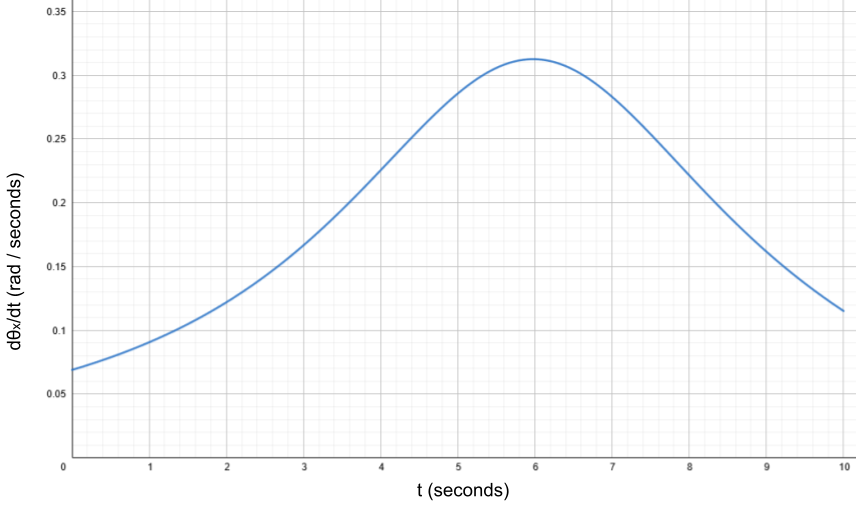
\includegraphics[width=500pt]{img/graph1.png}
\caption{\label{fig:3}Graph of $\dfrac{d\theta_x}{dt}$ vs time $t$}
\end{figure}

The motor rotating the camera about the x-axis will increase its speed of rotation until a local maxima at about 6 seconds, after which it will slow down, although the angle will still be increasing. I found this interesting because the local maxima, which translates to an inflection point in the graph of $\theta_x$ versus time, illustrates how the distance between the zipliner and camera decreases for the first half of the ride, and increases in the second half, hence the speeding up then slowing down of the rotation. 

\newpage 
Similarly, let's graph the rate of change of $\theta_y$ across time. 

\begin{figure}[H]
\centering
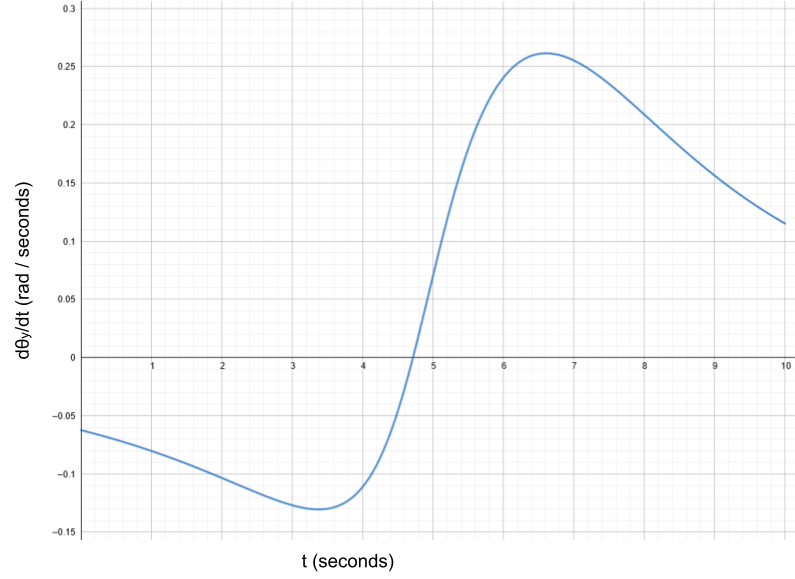
\includegraphics[width=500pt]{img/graph2.png}
\caption{\label{fig:4}Graph of $\dfrac{d\theta_y}{dt}$ vs time $t$}
\end{figure}

This is my favorite graph of the three because there is clearly a local minima and local maxima, and the angle is decreasing until around $4.7$ seconds, then increasing for the rest of the ride. Initially, I was expecting all the angles to always be increasing in speed, meaning that the rates of change would all have positive values. This is not necessarily the case, as shown with the rotation about the y-axis, as this motor would have to compensate for the rotation done by the motor rotating in the x-axis. So, even though the zipliner is traveling always towards the left ($y \to -\infty$), the angle between the y-axis is not strictly increasing. While at first this seemed counter-intuitive, it made sense when realizing that any rotation about the x-axis and z-axis also affects the orientation of $\vec n$ in the xy plane and yz plane. 

\newpage

Finally, let's graph the rate of change of $\theta_z$ across time. 
\begin{figure}[H]
\centering
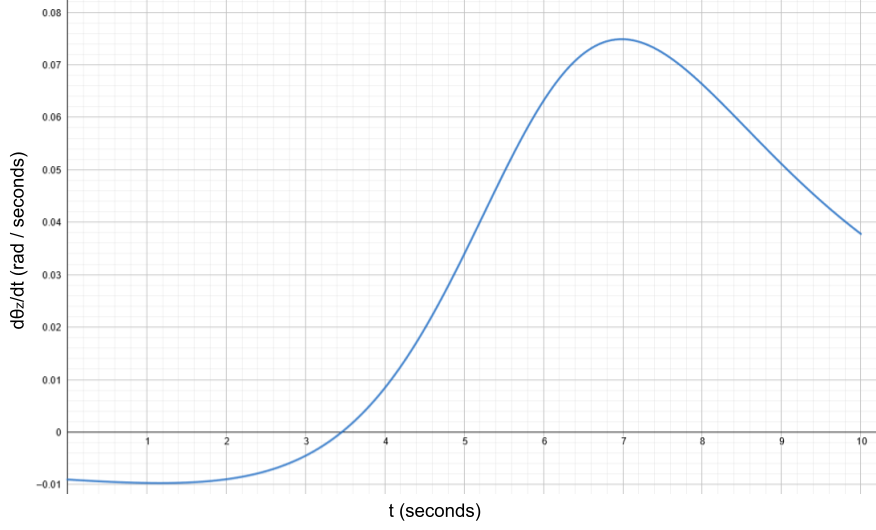
\includegraphics[width=500pt]{img/graph3.png}
\caption{\label{fig:5}Graph of $\dfrac{d\theta_z}{dt}$ vs time $t$}
\end{figure}

Again, we see that the angle initially decreases as they rate of change is negative, however after around $3.4$ seconds it begins to increase, then reach a local maxima and decrease in speed while still increasing the angle. This angle between $\vec n$ and the z-axis exhibits similar behavior to the previous two angles, as it will first decrease then increase to compensate for the angle about the x-axis increasing drastically in the first few seconds. This again emphasizes how any rotation between the three axis is dependent on the rotation around the other two axis.

\section{Conclusion}
The rates of change for the three angles defining the orientation of the camera to capture the zipliner as they travel down the zipline were successfully derived through a mixture of related rates calculus and 3-dimensional vectors. What was most fascinating about the results is that even though the zipliner moves in a straight line at constant velocity, the angles do not exhibit linear rotation, rather have far more complex behavior since they are affected by changes in position in the three dimensions. The final results were both shocking due to their complexity and pleasing because of the beauty in their insight into vector calculus. As intimidating as the evaluated equations in terms of time are, their vector form has striking, unexpected similarity. It is also interesting how all three angles have similar equations for their rates of change yet differ so drastically when viewed graphically, demonstrating both a pattern and discrepancy in the behavior of each motor rotating between the x, y, and z axis.
\subsection{Strengths}

A particular strength of this investigation is the use of vectors when finding the related rates. This allowed for the camera to be oriented in three dimensions, which is especially helpful for tracking any real-world objects which are not limited to two dimensional movement. 

Moreover, the equations derived for each angle and their rate of change can be used for any camera and zipline setup without restrictions to where it should be positioned. This is especially helpful if some tourists want a video with a mountain in the background or the river; simply modify the coordinates of point $C$. Similarly, any zipline can be evaluated regardless of its size by modifying coordinates $P_i$ and $P_f$. 

\subsection{Limitations}
The biggest limitation of this investigation is that it assumes the zipliner is traveling at constant velocity. This approximates the motion of a zipliner over time because high frictional forces result in the zipliners achieving terminal velocity that can be used as $\vec v$ \autocite{terminal}. However, gravity still plays a role in accelerating the zipliner as they travel, especially in the first few seconds of the descent. This results in the time axis in reality slightly deviating from my calculations, however, it has no effect on the overall behavior of the angles and their rates of change, only scales the time axis. 

% SOURCE; https://phys.libretexts.org/Courses/Joliet_Junior_College/Physics_201_-_Fall_2019/Book%3A_Physics_(Boundless)/6%3A_Applications_of_Newton/6.07%3A_Drag_Force_and_Terminal_Speed

\subsection{Extensions and Improvements}
An extension that was hinted at throughout the investigation was to instead use vector calculus to find the angles and their rates of change. This would provide more insight into the equations and the reason behind each variable. For example, if I created an angle-vector for angles $\theta_x$, $\theta_y$, and $\theta_z$, while in reality this would have no real-world meaning, it would showcase the the angles live in a unit sphere that Euler used to develop the concept of Euler Angles \autocite{euler}. 

Additionally, I would love to find the rates of change without constant velocity so that the camera always captures the zipliner in the center of the frame, even when accelerating. This extension would incorporate the acceleration vector into the equations which would undoubtedly make them more complex \autocite{acceleration}. 

\vspace{30pt}

This camera setup will make countless tourists at my Uncle's zipline park happy with unforgettable memories as their paralyzing fear of descending large ziplines is forever recorded for them to watch! Why use bad-quality cellphone videos if you can use 3D vector calculus instead?!

\newpage
\printbibliography

\end{document}
